\documentclass{beamer}
\usetheme{Malmoe}
\usepackage{comment}
\mode<presentation>{}
%% preamble
\title{Web Mining Tutorial}
\subtitle{Hadoop, Hive and Pig}
\author{Ajay Dubey, Romil Bansal, Jayant Gupta}

\begin{document}
%% title frame
\begin{frame}
\titlepage
\end{frame}

\begin{frame}{Doubt Clarification}
\begin{center}
\begin{itemize}
\item Text Indexing and Crawling
\item Relevance Ranking
\item Similarity Search
\item Link Analysis Algorithms
\item LSI and EM
\end{itemize}
 \end{center}
\end{frame}

\begin{frame}{Apache Hadoop Installation}
Pre-requisites 
\begin{center}
\begin{itemize}
\item Install Java 1.6 or above
\item Download Hadoop Version \textbf{1.2.1}
\item For Single Node Cluster \\ \href{http://www.michael-noll.com/tutorials/running-hadoop-on-ubuntu-linux-single-node-cluster/}{\beamergotobutton{http://www.michael-noll.com/tutorials/running-hadoop-on-ubuntu-linux-single-node-cluster/}}
\item For Multi Node Cluster \\ \href{http://www.michael-noll.com/tutorials/running-hadoop-on-ubuntu-linux-multi-node-cluster/}{\beamergotobutton{http://www.michael-noll.com/tutorials/running-hadoop-on-ubuntu-linux-multi-node-cluster/}}
\end{itemize}
 \end{center}
\end{frame}

\begin{frame}{Apache Hadoop Configurations}
\begin{center}
In configurations folder  (HADOOP-HOME/conf) make changes in
\begin{itemize}
\item hadoop-env.sh
\item core-site.xml
\item mapred-site.xml
\item hdfs-site.xml
\end{itemize}
 \end{center}
\end{frame}

\begin{frame}{Apache Hadoop Configurations cont.}
For multi node cluster setup 
\begin{itemize}
\item make changes in folder (HADOOP-HOME/conf)
\begin{itemize}
\item masters
\item slaves
\end{itemize}
\item in /etc folder
\begin{itemize}
\item hosts file must contain IP addresses of masters and slave machines
\end{itemize}
\item ssh access from master to slave without password
\end{itemize}
\end{frame}

\begin{frame}{Hadoop cont.}
\begin{itemize}
\item bin/hadoop namenode -format
\item bin/start-dfs.sh
\item bin/start-mapred.sh
\item bin/hadoop dfs -ls
\item bin/hadoop dfs -copyFromLocal $\langle$local-dir$\rangle$ $\langle$hdfs-dir$\rangle$
\item bin/hadoop dfs -copyToLocal $\langle$hdfs-dir$\rangle$ $\langle$local-dir$\rangle$
\item bin/hadoop jar hadoop-examples-1.2.1.jar wordcount data output
\end{itemize}
\end{frame}

\begin{frame}{Map Reduce Architecture}
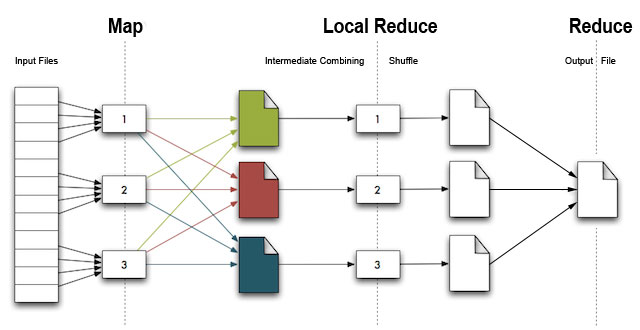
\includegraphics[width=0.9\textwidth]{images/1.jpg} 
\end{frame}

\begin{frame}{Word Count Example}
Map Function
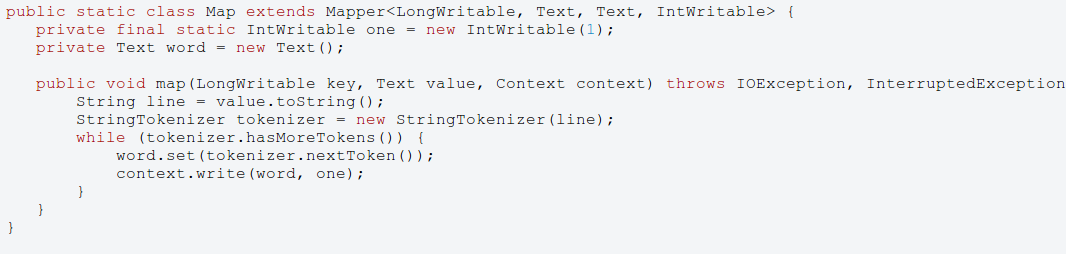
\includegraphics[width=1.4\textwidth]{images/2.png} 
\\
Reduce Function
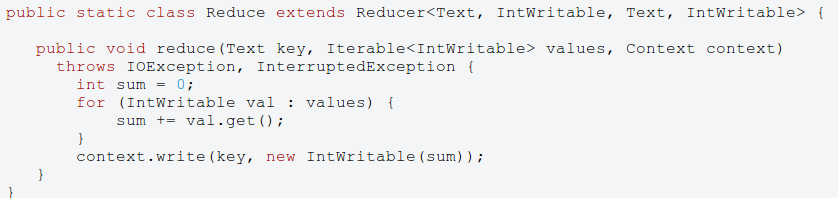
\includegraphics[width=1.3\textwidth]{images/3.png} 
\end{frame}

\begin{frame}{Jar File Creation}
Export as a jar file and use class name containing both Map and Reduce
\end{frame}

\begin{frame}{Apache Pig}
Installation
\begin{itemize}
\item Download Apache Pig Version \textbf{0.11.1}
\item export PATH of your PIG-Home
\end{itemize}
Execution
\begin{itemize}
\item Local Mode \\ pig -x local
\item Map Reduce Mode \\ pig OR pig -x mapreduce
\end{itemize}
\end{frame}


\begin{frame}{Apache Pig}
Installation
\begin{itemize}
\item Download Apache Pig Version \textbf{0.11.1}
\item export PATH of your PIG-Home
\end{itemize}
Execution
\begin{itemize}
\item Local Mode \\ pig -x local
\item Map Reduce Mode \\ pig OR pig -x mapreduce
\end{itemize}
\end{frame}

\begin{frame}{Apache Pig cont.}
Pig Latin Statements
\begin{itemize}
\item A LOAD statement reads data from the file system.
\item A series of "transformation" statements process the data.
\item A STORE statement writes output to the file system; or, a DUMP statement displays output to the screen.
\end{itemize}
\end{frame}

\begin{frame}{Apache Hive}
Installation
\begin{itemize}
\item Download Apache Hive Version \textbf{0.10.0}
\item export PATH of your HIVE-Home
\end{itemize}
Execution (only in Map Reduce way)
\begin{itemize}
\item hive
\end{itemize}
\end{frame}

\begin{frame}{Apache Hive Commands}
Hive Commands
\begin{itemize}
\item hive: SHOW TABLES;
\item hive: CREATE TABLE wordcount (words STRING, count INT) ROW FORMAT DELIMITED FIELDS TERMINATED BY tab STORED AS TEXTFILE;
\item hive: DESCRIBE wordcount;
\item hive: LOAD DATA INPATH “words” INTO TABLE wordcount;
\item hive: LOAD DATA LOCAL INPATH …
\end{itemize}
\end{frame}

\begin{frame}{Apache Hive Advanced Features}
“TRANSFORM:” Allows user to stream data through user-defined scripts. \\
user: cat split.py\\
for line in sys.stdin:\\
	for word in line.split():\\
		print word\\
		Add file split.py\\
INSERT OVERWRITE TABLE test\\
SELECT TRANSFORM(line)\\
USING ‘python split.py’\\
AS word\\
FROM wordcount;\\
\end{frame}

\begin{frame}{References}
\begin{center}
\begin{itemize}
\item \href{http://hadoop.apache.org/docs/stable/mapred_tutorial.html}{\beamergotobutton{Apache Hadoop Map Reduce Tutorial}}
\item \href{http://pig.apache.org/docs/r0.7.0/tutorial.html}{\beamergotobutton{Apache Pig Installation}}
\item \href{http://pig.apache.org/docs/r0.8.1/piglatin_ref1.html}{\beamergotobutton{Apache Pig Reference Manual 1}}
\item \href{http://pig.apache.org/docs/r0.8.1/piglatin_ref2.html}{\beamergotobutton{Apache Pig Reference Manual 2}}
\item \href{http://blog.cloudera.com/wp-content/uploads/2010/01/6-IntroToHive.pdf}{\beamergotobutton{Introduction to Hive}}
\item \href{https://cwiki.apache.org/confluence/display/Hive/Tutorial}{\beamergotobutton{Apache Hive Tutorial}}
\end{itemize}
\end{center}
\end{frame}

\begin{frame}
\begin{center}
Thank You
\end{center}
\end{frame}

\end{document}